 \documentclass{report}
 
\usepackage[utf8]{inputenc} 
\usepackage[T1]{fontenc}      
\usepackage[top=2.0cm, bottom=3cm, left=3.0cm, right=3.0cm]{geometry}
\usepackage{graphicx}
\usepackage{wrapfig}
\usepackage{amsmath,esint }
\usepackage{amssymb}
\graphicspath{{figures/}{../figures}}

\newcommand*\dif{\mathop{}\!\mathrm{d}}
\newcommand*\diver{\mathop{}\!\mathrm{div}}
\newcommand*\grad{\mathop{}\!\mathrm{grad}}

\begin{document}

\section*{Exercice 1}

On considère un fil unidimensionnel de section $\Sigma$ dirigé suivant l'axe $x$. Il est constitué d'atomes séparés d'une distance $a$, de charge $+e$  et d'autant d'électrons de conduction de charge $-e$ ; on suppose que atomes et électrons sont confondus sur l'axe $x$ et uniformément répartis à travers $\Sigma$. On impose un courant $I$ dans le fil, les électrons se déplacent alors avec une vitesse $\vec{v'}=v'\vec{e_{x}}$.

Une particule de charge $q$ se déplace à la vitesse $\vec{v}=v\vec{e_{x}}$ à une distance $r$ de l'axe $x$, supérieure au rayon du fil.

\begin{figure}[h!]
\centering
		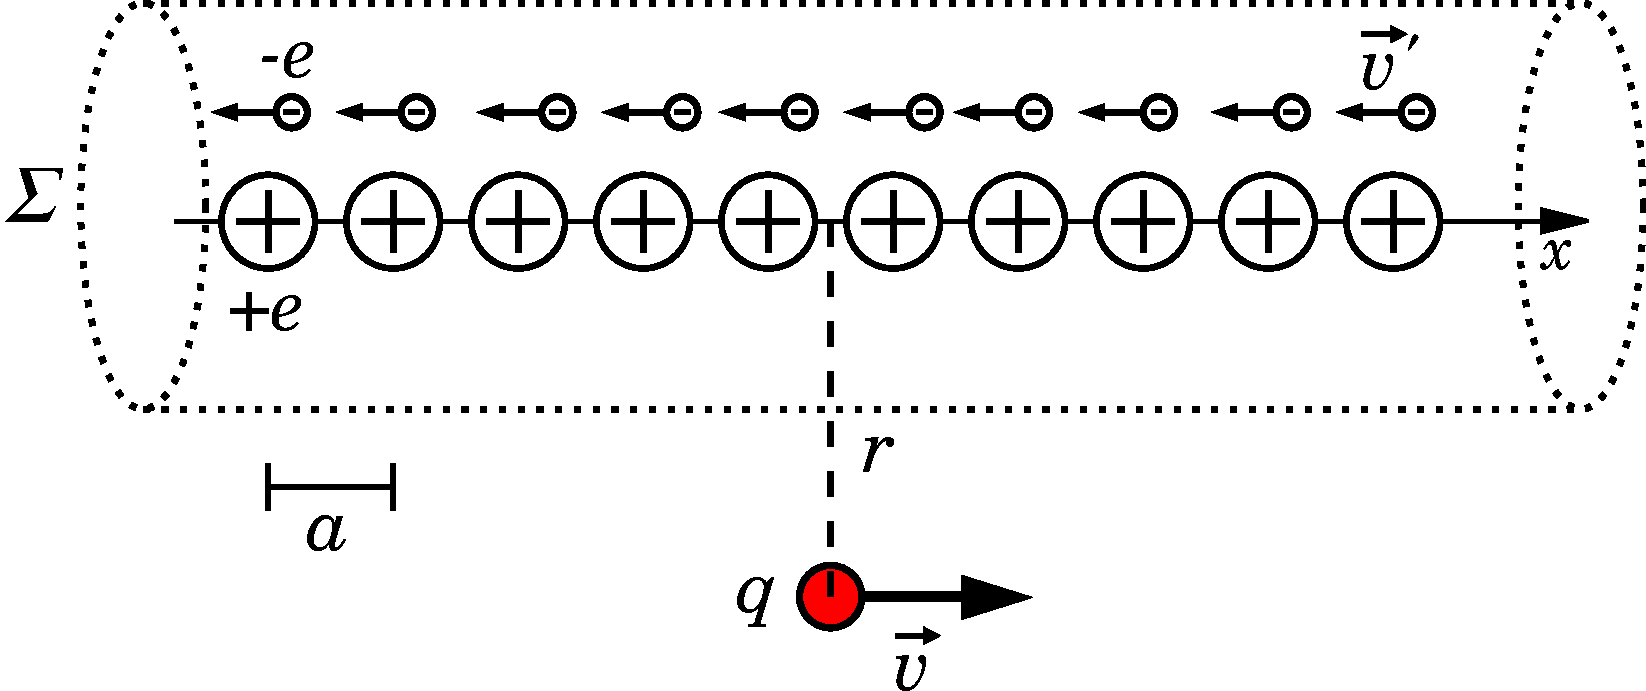
\includegraphics[scale=0.25]{cable.pdf}
\end{figure}

On s'intéresse aux forces électromagnétiques exercées par les charges du fil sur la particule de charge $q$ par deux approches différentes.

\subsubsection*{Approche en mécanique classique}

\begin{itemize}
	\item[$\clubsuit$] Quelle est la densité de charge $\rho_{+}$ (respectivement $\rho_{-}$) due aux atomes (resp. aux électrons) dans le fil ? 
	
	\item[$\clubsuit$] Quel est la densité de courant $\vec{j}$ dans le fil ? Exprimer la vitesse $\vec{v'}$ des électrons de conduction en fonction de $I$.
	
	\item[$\clubsuit$] Quel est le champ électrique créé par la distribution de charges ? 
	\item[$\clubsuit$] Quel est le champ magnétique créé par le courant $I$ ?
		\item[$\clubsuit$] Quelle est la force totale s'exerçant alors sur la charge $+q$ ? Quels sont les contributions des forces électriques et magnétiques sur cette particule ?
\end{itemize}

\subsubsection*{Approche en mécanique relativiste}

En relativité restreinte, tout objet se déplaçant relativement par rapport à un autre voit sa longueur contractée dans le sens du déplacement. Ainsi, Einstein a démontré en 1905 qu'un objet à la vitesse $v$ par rapport à un autre objet, voit la longueur de ce dernier contracté du facteur $\gamma=1/\sqrt{1-v^{2}/c^{2}}$ (où $c$ est la vitesse de la lumière). La charge $q$ voit donc la densité de charge des atomes $\rho_+$ et des électrons $\rho_-$ augmenter, mais pas dans les mêmes proportions. 
	\begin{itemize}
		\item[$\clubsuit$] Que deviennent les densités de charge $\rho_{+}$ et $\rho_{-}$ dans le référentiel de la particule $+q$ ? On admettra que les électrons se déplacent à la vitesse $v'-v$ dans le référentiel de $+q$. 
		\item[$\clubsuit$] Déterminer le champ électrique créé par cette nouvelle distribution de charges. 
		\item[$\clubsuit$] Quelle est la force électrique s'exerçant sur la particule $+q$ ? On supposera que $v'\ll v\ll c$.
		\item[$\clubsuit$] Comparer avec le résultat trouvé en approche classique (non relativiste).
	\end{itemize}
			
\textit{N.B.} : On rappelle que la vitesse de la lumière $c$ est définie comme $c^{2}=1/\epsilon_{0}\mu_{0}$, où $\epsilon_{0}$ et $\mu_{0}$ sont respectivement la permittivité électrique et la perméabilité magnétique du vide.

\newpage

\section*{Exercice 2}

\subsubsection*{Corrosion uniforme du zinc en milieu acide}

\begin{itemize}

	\item[$\clubsuit$] Donner l'allure de la courbe densité de courant - potentiel pour l'oxydation et la réduction du couple $Zn/Zn^{2+}$. Ce couple est rapide. Le potentiel standard du couple est -0,76V et on prendra une concentration initiale d'ions zinc II égale à 1 mol.L$^{-1}$.
	
	\item[$\clubsuit$] La courbe intensité-potentiel du couple $H^+/H_2$ dépend-elle du métal utilisé ? Expliquer pourquoi.
	
	\item[$\clubsuit$] On envisage la réduction du zinc par les ions $H^+$. Ecrire l'équation de la réaction. Que peut-on dire de cette oxydation par des considérations thermodynamiques ?

\end{itemize}

Pour des valeurs importantes de la valeur absolue de la densité de courant anodique $\mid j_a\mid$ (resp. cathodique $\mid j_c\mid$), on peut écrire : $j_a=A_a\exp(b_aE)$ et $j_c=-A_c\exp(-b_cE)$. La constante $b_a$ (resp. $b_c$) est positive et caractéristique de l'oxydant (resp. du réducteur). Les constantes $A_a$ et $A_c$ sont positives et dépendent des activités de l'oxydant et du réducteur.

On envisage le phénomène de corrosion uniforme, observée lorsqu'une lame de zinc trempe dans la solution acide. On admet alors que les surfaces d'électrodes sont égales pour l'oxydation et la réduction. 

\begin{itemize}

	\item[$\clubsuit$] Quelle est la relation entre les intensités anodiques et cathodiques ? Que peut-on en déduire sur les densités de courants ?
	
	\item[$\clubsuit$] Une étude expérimentale a permis d'obtenir les lois suivantes, reliant la densité de courant et le potentiel d'électrode mesuré par rapport à l'ESH (les grandeurs sont en unités SI) :
	\begin{itemize}
		\item[-] Oxydation du zinc : $E=0,0774\log_{10}(j_a)-0,1956$
		\item[-] Réduction de $H^+$ sur zinc : $E=-0,0780\log_{10}(\mid j_c\mid)-0,778$
	\end{itemize}
Calculer la densité de courant de corrosion uniforme $j_{corr}$ et le potentiel de corrosion $E_{corr}$.

	\item[$\clubsuit$] La vitesse de corrosion est mesurée en $\mu$m par années. Exprimer littéralement $v_{corr}$ en fonction de $j_{corr}$, de la constante de Faraday $F$, de la masse atomique du zinc et de sa masse volumique. Application numérique : $M_{Zn}=65,4$g.mol$^{-1}$, $\rho_{Zn}=7140$kg.m$^{-3}$ et $F=96490$C.mol$^{-1}$.
\end{itemize}

\subsubsection*{Comparaison avec la corrosion du fer}

\begin{itemize}
	
		\item[$\clubsuit$] On donne $E^0=-0,44$V pour le couple $Fe/Fe^{2+}$. A partir de considérations thermodynamiques, quel métal serait le plus corrodé par la même solution acide ?
		
	\item[$\clubsuit$] Une étude expérimentale, réalisée dans les mêmes conditions, a permis d'obtenir :
	\begin{itemize}
		\item[-] Oxydation du fer : $E=0,0760\log_{10}(j_a)-0,0348$
		\item[-] Réduction de $H^+$ sur fer : $E=-0,0780\log_{10}(\mid j_c\mid)-0,476$
	\end{itemize}
	Calculer la densité de courant de corrosion uniforme du fer et conclure.
		
	\item[$\clubsuit$] Représenter grossièrement les graphes $E(\log j)$ pour l'oxydation du zinc, la réduction de $H^+$ sur zinc, l'oxydation du fer, la réduction de $H^+$ sur fer. On se limitera aux valeurs de $E$ comprises entre 0 et-1V et de $\log j$ comprises entre 0 et -5.
	
	\item[$\clubsuit$] Deux blocs, l'un de fer et l'autre de zinc de même surface et reliés électriquement, sont plongés dans la solution acide précédente. Décrire les phénomènes observés, indiquer quel métal sera le plus corrodé et calculer la densité de courant. Conclure. 
	
\end{itemize}

\newpage

\section*{Exercice 3}

En 1900, Paul Drude proposa un modèle permettant d'expliquer les propriétés de conduction électrique et thermique des métaux. Dans ce modèle, on considère que les électrons de conduction forment un gaz de particules classiques de masse $m$ et de charge $-e$, auquel on applique les méthodes issues de la théorie cinétique des gaz. Les électrons effectuent des collisions, considérées comme instantanées. Ils sont supposés indépendants (pas d'interaction électron-électron entre les collisions). Drude attribua les collisions aux chocs entre les électrons et les ions, plutôt qu'aux chocs entre les électrons entre eux comme pour un gaz ordinaire. À l'issue d'une collision, la vitesse de l'électron a une direction aléatoire (pas de direction privilégiée), et une valeur liée à la température à l'endroit où a lieu la collision.

\subsubsection*{Temps de relaxation}

Le paramètre fondamental du modèle de Drude est le temps de collision  $\tau$ ou temps de relaxation. Il représente la durée moyenne entre deux collisions. En d'autres termes, pour un électron donné, la probabilité de subir une collision pendant un intervalle de temps infinitésimal $dt$ est $dt/\tau$. On notera $N_0$ la population totale d'électrons.

\begin{itemize}
	
	\item[$\spadesuit$]	 Montrer que pour un électron donné, observé à l'instant $t=0$, la probabilité de $P(t)$ de ne pas subir de collision est $\exp(-t/\tau)$. 
	
	\item[$\spadesuit$] On soumet le métal à un champ de force extérieur, et on note $\vec{F}(t)$ la force subie par chaque électron. Comment varie la quantité de mouvement de la totalité des électrons $\vec{P}(t)$ entre $t$ et $t+dt$ ?
	
	\item[$\spadesuit$] En déduire une équation différentielle vérifiée la vitesse moyenne d'un électron $\vec{v}=\vec{P}/(mN_0)$. Quel est l'effet moyen des collisions sur la trajectoire d'un électron ?
	
	\item[$\spadesuit$] On applique au métal un champ électrique uniforme de pulsation $\omega_0$, que l'on note en notation complexe : $\vec{E}(t)=E_0\exp(-i\omega_0t)$. En appliquant le résultat précédent, calculer la densité de courant $\vec{j}$ en fonction de $m$, $e$, $\tau$ et du nombre d'électrons par unité de volume $n$. En déduire l'expression de la conductivité $\gamma(\omega)$ du métal.
	
	\item[$\spadesuit$] En admettant que chaque atome du métal libère un électron de conduction, calculer un ordre de grandeur de $n$.
	
	\item[$\spadesuit$] La résistivité statique du cuivre est mesurée à 273K est $\rho=1,56\cdot10^{-8}\Omega$.m. Calculer le temps de relaxation $\tau$. 
	
	\item[$\spadesuit$] A $t=0$, on applique un champ $\vec{E}$ constant aux électrons du conducteur. Quelle est l'évolution de la vitesse moyenne au cours du temps ? 
\end{itemize}

\newpage

\section*{Exercice 4}

On considère une plaque métallique de conductivité $\gamma$, infinie dans le plan $xy$ et d'épaisseur $e$ selon $z$. Cette plaque est connectée à deux fils de même métal (et donc de même conductivité $\gamma$) en $A$ et $B$, séparés l'un de l'autre de la distance $d$. Ces deux fils peuvent être assimilés à des cylindres de rayon $a$ et de longueur $l$. 

\begin{figure}[h!]
\centering
		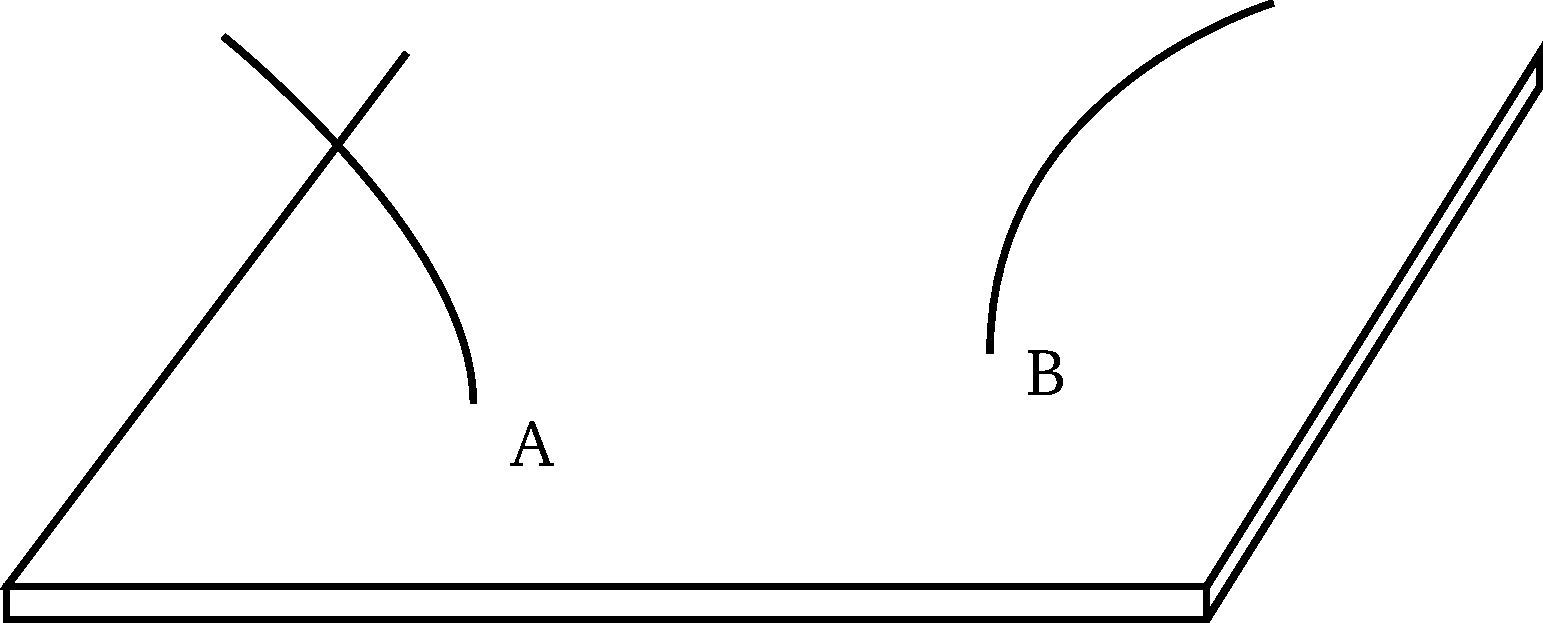
\includegraphics[scale=0.3]{plaque.pdf}
\end{figure}

\begin{itemize}

	\item[$\heartsuit$] Quelle est la résistance de chaque fil ? 
	
	\item[$\heartsuit$] A l'aide des symétries du problème, proposez une expression pour la densité de courant à l'intérieur de la plaque. 
	
	\item[$\heartsuit$] En déduire la résistance équivalente entre les points $A$ et $B$. Quelle est la résistance totale du dispositif ?
	
	\item[$\heartsuit$] On considère désormais que les fils sont reliés ne sont plus reliés à une plaque mais à un volume du même métal, c'est-à-dire, $e\longrightarrow\infty$. Par le même raisonnement, en déduire la résistance équivalente. 

\end{itemize}

\newpage

\section*{Exercice 5}

Lorsque le courant de foutre d'un impact direct sur un paratonnerre s'écoule par la prise de terre d'une installation, de fortes surtensions peuvent apparaître. La résistance de prise de terre ne doit pas dépasser 30$\Omega$. Considérons une prise de terre constituée d'une demi-sphère métallique pleine, de rayon $a$ et placée dans un sol de conductivité $\gamma\approx10^{-2}$S.m$^{-1}$. Le courant de foudre d'intensité $I$ arrive sur la tige paratonnerre fixée au centre $C$ de l'hémisphère.

\begin{figure}[h!]
\centering
		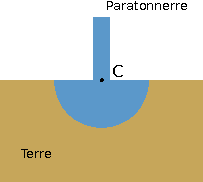
\includegraphics[scale=1.5]{EM1.pdf}
\end{figure}

\begin{itemize}
	
	\item[$\diamondsuit$] Quelle est la densité de courant $\vec{j}$ dans le sol pour $r>a$ ? Déterminer alors le potentiel $V(r)$, en supposnat que celui-ci est nul à l'infini. 
	
	\item[$\diamondsuit$] Déterminer la valeur du rayon $a$ pour laquelle la valeur de la résistance de la prise de terre ne dépasse pas 30$\Omega$.
	
	\item[$\diamondsuit$] La tension de pas est définie comme la différence de potentiel entre 2 points de la surface du sol distants de 1 mètre et situés sur la même droite issue du centre $C$ de l'hémisphère. Calculer cette tension de pas $V_p$ pour un courant de 50kA, à une distance de 10m puis de 100m.
	
	\item[$\diamondsuit$] Sachant que la résistance entre les deux pieds d'une personne est de l'ordre de 2500$\Omega$, et que l'intensité létale pour un corps humais est de 25mA, une personne est-elle en sécurité à 10m ? A 100m ? 
	
\end{itemize} 

\newpage

\section*{Câble coaxial}

On considère un câble coaxial constitué de deux conducteurs cylindriques de même axe, de rayon $a$ (l'âme) et $b$ (la gaine), avec $a<b$, et d'épaisseur négligeable. Le conducteur central (de rayon $a$) a une charge surfacique $\sigma_a$ et est traversé par une densité surfacique de courant $\vec{j_{s,a}}$. La longueur du câble est $L$, très grande devant les rayons $a$ et $b$.  

\begin{figure}[h!]
\centering
		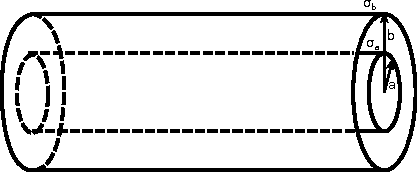
\includegraphics[scale=1]{em2.pdf}
\end{figure}

On cherche à connaitre la capacité et l'inductance linéique du câble coaxial, pour comprendre la propagation des ondes électromagnétiques à l'intérieur. 

\begin{itemize}

	\item[$\blacksquare$] Exprimer le courant $I$ circulant dans l'âme et sa charge totale $Q$ en fonction de $\vec{j_{s,a}}$ et $\sigma_a$. En déduire la charge et l'intensité surfacique de la gaine, $\sigma_b$ et $\vec{j_{s,b}}$, sachant que le courant total à travers le câble est nul et qu'il est neutre électriquement.
	
	\item[$\blacksquare$] Déterminer le champ électrique en tout point.

	\item[$\blacksquare$] En déduire la capacité $c$ par unité de longueur de câble. 
	
	\item[$\blacksquare$]	 Déterminer le champ magnétique en tout point. 
	
	\item[$\blacksquare$] On définit l'inductance $L$ d'un circuit délimitant une surface $S$, parcouru par un courant $I$ comme  comme le rapport du flux du champ magnétique à travers $S$ avec le courant $I$ :
	\begin{align*}
		\Phi_B=\oiint_S \dif \vec{S}\cdot\vec{B}=LI
	\end{align*}
En choisissant soigneusement une surface $S$, déterminer l'inductance linéique $l$. 

	\item[$\blacksquare$] Que vaut le produit le produit $l\times c$ ? A quoi correspond cette grandeur ?
	
\end{itemize}

\newpage

\section*{Étude d'un colloïde}

Les colloïdes sont constitués par un solvant dans lequel est introduit un corps, généralement solide, qui se disperse sous forme de particules en suspension dont la taille peut varier de 10 à 100nm. Ces particules sont des macromolécules ou des agrégats de petites molécules qui s'ionisent dans le milieu. Par exemple, le blanc d'œuf ou le plasma sanguin sont des solutions colloïdales. En agronomie, le colloïde formé par les particules d'argile (silice) et l'humus (matière organique décomposée) est fondamental pour la fertilité des sols. 

On supposera que la solution colloïdale est composée de :
\begin{itemize}
	\item[-] des particules de colloïdes, de rayon $r_0$, portant une charge $Q$ sur leur surface. Ils sont supposés assez dilués pour considérer que le potentiel autour d'une particule colloïdale n'est créé que par elle-même et les ions du milieu ;
	
	\item[-] les ions contenus dans l'eau, supposés ponctuels, portant une charge $\pm e$ à la concentration $N_0$. On supposera que la concentration en cations est égale à celle en anion. Les ions (cations + ou anions -), quand il sont soumis à un potentiel V, se répartissent en moyenne selon la loi de Boltzmann :
\begin{align*}
	\frac{N_{\pm}(r)}{N_0}=\exp\left(-\frac{\pm eV(r)}{k_BT} \right) 
\end{align*}
La permitivité du milieu est $\varepsilon=\varepsilon_r\varepsilon_0$ avec $\varepsilon_r=80$.
\end{itemize}

Lorsqu'on augmente significativement la concentration $N_0$ de la solution ionique, on observe que la suspension colloïdale sédimente très rapidement. On cherche à comprendre ce phénomène appelé \textit{floculation}. Pour cela, on s'intéresse à une particule de colloïde en suspension dans la solution, entourée des ions. 

\begin{itemize}

	\item[$\heartsuit$] Établir la densité volumique de charge entourant une particule de colloïde. Que devient cette expression si $eV\ll k_BT$ ?
	
	\item[$\heartsuit$] En appliquant le théorème de Gauss sur un volume bien choisi, montrer que : 
	\begin{align*}
		\frac{1}{r}\frac{\dif}{\dif r}\left( r^2\frac{\dif V}{\dif r}\right) +\frac{\rho}{\epsilon}=0
	\end{align*}

	\item[$\heartsuit$] Résoudre l'équation différentielle en posant $U(r)=rV(r)$, et retrouver l'expression de $V(r)$, en fonction de $r$, une longueur caractéristique $\lambda$ et une constante d'intégration qu'on ne cherchera pas à définir. Donner un ordre de grandeur de $\lambda$ à température ambiante dans de l'eau pure.
	
	\item[$\heartsuit$] Écrire l'expression du champ électromagnétique. En déduire la constante d'intégration, et l'expression de $V(r)$. 
	
	\item[$\heartsuit$] Quelle est l'expression de la densité de charge $\rho$ ? Justifier l'appellation d'\textit{écrantage}.
	
	\item[$\heartsuit$] Quelle est la force $F(d)$ qui s'exerce entre deux particules de colloïde éloignées d'une distance $d$ ? Comparer cette force dans le cas d'une eau pure et celle d'une électrolyte de concentration $N_0=100$. Pourquoi parle t-on de coagulation ?

\end{itemize} 

\newpage

\section*{Condensateur Terre-ionosphère}

On représente l'ensemble Terre-ionosphère comme un volumineux condensateur sphérique. La Terre, de rayon $R$, se comporte comme un conducteur parfait de potentiel nul et porte une charge négative $-Q$, uniformément répartie sur sa surface, tandis que la ionosphère est représentée par une surface équipotentielle sphérique de rayon $R+z_0$, de potentiel $V$ possède une charge totale $+Q$. On suppose que la permittivité de l'atmosphère est celle du vide, soit $\varepsilon_0$. 

\begin{figure}[h!]
\centering
		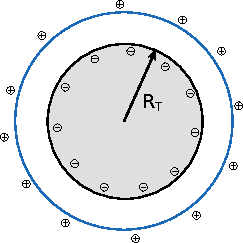
\includegraphics[scale=1]{em3.pdf}
\end{figure}

\begin{itemize}
	
	\item[$\clubsuit$] Déterminer le champ électrique $\vec{E}$.
		
	\item[$\clubsuit$] En déduire la capacité $C$ du système Terre-ionosphère.
	
	\item[$\clubsuit$] Des mesures ont permis de déterminer le potentiel de l'ionosphère à l'altitude $z_0=60$km à environ 360kV. Justifier que le système se comporte comme un condensateur plan. Quel est la valeur de la capacité $C$ et l'énergie électrostatique du système $W_{el}$, ainsi que la valeur du champ électrique au niveau du sol.
	
	\item[$\clubsuit$] Donner la valeur de la densité de charge $\sigma$ à la surface de la Terre. Quelle est la charge totale $-Q$ ?
	
	\item[$\clubsuit$] Lors d'un orage, les mouvements convectifs de l'air font passer la tension augmentent fortement la tension entre le sol et le bas des nuages. Les éclairs apparaissent lorsque le champ électrique dépasse un seuil, appelé \textit{champ disruptif} : l'air s'ionise et devient conducteur. Sachant que pour un air humide, ce champ disruptif est de $E_{dis.}\simeq10^{5}$V.m$^{-1}$. A quelle tension $V_1$ observe t-on l'apparition des éclairs ?
	
	
	\textit{Données} : Rayon de la Terre, $R_T=6370$km. Permittivité du vide, $\varepsilon=8,85\cdot10^{-12}$F.m$^{-1}$.
	
\end{itemize}

\newpage

\section*{Exercices en pagaille}

\begin{itemize}

	\item[$\spadesuit$] On considère une boule métallique de rayon $R$. A l'instant $t$, on la monte instantanément au potentiel $V$. Quel est la charge $Q$ de la sphère ? Justifier qualitativement que la charge se répartit sur la surface de la sphère.
	
	\item[$\spadesuit$] On considère un plan infini, avec une charge surfacique $\sigma$. Quel est le champ électrique en tout point de l'espace ? Justifier la présence d'une discontinuité du champ. 
	
	\item[$\spadesuit$] Quel est le champ magnétique créé par une nappe de courant infiniment fine parcouru par une densité de courant $\vec{j_s}$ ? 
	
	\item[$\spadesuit$] A l'aide du théorème d'Ampère, déterminer le champ créé par une bobine de $N$ spires, de longueur $L$ et de rayon $R$, avec $L\gg R$.
	
	\item[$\spadesuit$] On considère un tube parcouru par un courant de densité uniforme $\vec{j}$. Expliquer le phénomène de magnétostriction. On rappelle l'expression de la force de Laplace : $f_{vol}=\vec{j}\dif\tau\wedge\vec{B}$
	
\end{itemize}

\end{document}
